\documentclass[12pt,letterpaper]{article}

% ============================================================================
% PACKAGES
% ============================================================================
\usepackage[utf8]{inputenc}
\usepackage[T1]{fontenc}
\usepackage{amsmath,amssymb,amsthm}
\usepackage{mathtools}
\usepackage{graphicx}
\usepackage{booktabs}
\usepackage{natbib}
\usepackage{hyperref}
\usepackage{xcolor}
\usepackage{setspace}
\usepackage[margin=1in]{geometry}
\usepackage{caption}
\usepackage{subcaption}
\usepackage{float}
\usepackage{tikz}
\usetikzlibrary{arrows.meta,positioning,shapes.geometric,calc}
\usepackage{enumitem}
\usepackage{appendix}

% ============================================================================
% THEOREM ENVIRONMENTS
% ============================================================================
\theoremstyle{plain}
\newtheorem{hypothesis}{Hypothesis}
\newtheorem{proposition}{Proposition}
\newtheorem{lemma}{Lemma}
\newtheorem{corollary}{Corollary}

\theoremstyle{definition}
\newtheorem{definition}{Definition}
\newtheorem{assumption}{Assumption}
\newtheorem{remark}{Remark}

% ============================================================================
% CUSTOM COMMANDS
% ============================================================================
\newcommand{\E}{\mathbb{E}}
\newcommand{\R}{\mathbb{R}}
\newcommand{\Var}{\mathrm{Var}}
\newcommand{\Cov}{\mathrm{Cov}}
\newcommand{\rank}{\mathrm{rank}}
\newcommand{\tr}{\mathrm{tr}}
\newcommand{\SDF}{m}
\newcommand{\deff}{d_{\text{eff}}}

% ============================================================================
% HYPERREF SETUP
% ============================================================================
\hypersetup{
    colorlinks=true,
    linkcolor=blue!70!black,
    citecolor=blue!70!black,
    urlcolor=blue!70!black
}


\title{Macroeconomic Shocks, Arbitrage Constraints, and the
Time-Varying Effective Dimension of Asset Returns}

\author{
    Bernd J.\ Wuebben\\
    AllianceBernstein, New York\\ \texttt{bernd.wuebben@alliancebernstein.com}
}


\date{January 17, 2026}


% ============================================================================
% DOCUMENT
% ============================================================================
\begin{document}

\maketitle



\begin{abstract}
\noindent
Why does the ``factor zoo'' appear episodically rather than permanently? I propose that the effective dimension of asset returns---the number of independently priced directions in the stochastic discount factor---varies systematically with macroeconomic conditions. Using externally identified macroeconomic shocks, I document that contractionary shocks expand the effective dimension of returns, but only when arbitrage constraints bind. This dimension expansion explains why portfolios sorted on characteristics unrelated to systematic risk earn positive returns during stress periods: they load on pricing kernel directions that are dormant in normal times but become activated when arbitrage capital is scarce. The framework unifies anomaly timing, factor crowding, and limits-to-arbitrage phenomena under a single economic mechanism. Rather than treating mispricing as noise or behavioral error, I show it reflects a structured response of the pricing kernel to macroeconomic conditions operating through arbitrage constraints. These findings have direct implications for understanding why factor strategies exhibit pronounced time-variation in performance and suggest that factor zoo proliferation reflects state-dependent dimension of asset markets rather than measurement error or data mining.
\end{abstract}

\vspace{0.5cm}

\noindent\textbf{Keywords:} Effective dimension, stochastic discount factor, macroeconomic shocks, arbitrage constraints, anomalies, factor zoo

\vspace{0.3cm}

\noindent\textbf{JEL Classification:} G12, G14, E32, E44


\doublespacing

% ============================================================================
% 1. INTRODUCTION
% ============================================================================
\section{Introduction}\label{sec:intro}

Asset pricing theory offers a stark prediction: the stochastic discount factor (SDF) determines which risks are priced. Any return unexplained by exposure to priced risks represents either measurement error or a failure of the model. Yet decades of empirical research have produced a ``factor zoo'' of characteristics that predict returns without obvious links to systematic risk. The conventional response has been either to expand the factor model or to attribute these patterns to behavioral biases and market frictions. Neither approach addresses a more fundamental question: why does the apparent complexity of asset pricing vary over time?

This paper explains why the effective dimension of asset returns expands episodically.

I define effective dimension as the number of independently priced directions in the SDF. In a world with a single priced risk, all expected returns load on a single factor, and the cross-section of returns is effectively one-dimensional regardless of how many assets trade. When multiple risks are priced, the effective dimension increases, and the factor model required to explain returns becomes correspondingly more complex. The contribution of this paper is to identify the economic mechanism that causes effective dimension to change: exogenous macroeconomic shocks temporarily activate additional pricing kernel directions when arbitrage constraints bind.

The theoretical intuition follows from combining two established ideas. First, the SDF admits multiple potential sources of priced risk, but not all are active at all times. Some risks may have zero prices in normal conditions because arbitrageurs efficiently eliminate any premium associated with those exposures. Second, arbitrage capacity is finite and state-dependent. When macroeconomic shocks deplete arbitrage capital, previously well-arbitraged return patterns can no longer be eliminated, and their associated risk prices become economically relevant.

The empirical framework proceeds in three steps. First, I measure effective dimension directly using the covariance structure between returns and SDF innovations, building on the methodology of \cite{kozak2018interpreting}. Second, I show that effective dimension increases systematically following contractionary macroeconomic shocks, using externally identified monetary policy and fiscal shocks to establish causality. Third, I demonstrate that this dimension expansion occurs only when arbitrage constraint measures indicate that intermediary capital is scarce, confirming the proposed mechanism.

The results rationalize several puzzling features of the anomaly literature. Mispricing portfolios earn positive returns precisely when effective dimension is high, consistent with their loading on conditionally priced directions. Risk factors show no such state-dependence, consistent with their loading on always-priced directions. The episodic nature of factor zoo returns follows directly: these strategies exploit pricing kernel directions that are priced only intermittently.

This paper makes three contributions. First, I provide causal evidence on the determinants of effective dimension, moving beyond documentation to explanation. The use of externally identified shocks rules out reverse causality and simultaneity concerns that plague most studies of time-varying risk premia. Second, I unify anomaly timing, factor crowding, and limits-to-arbitrage literatures under a common framework. The mechanism is dimension expansion, not simply risk premium variation. Third, I offer a precise diagnostic for when mispricing returns are economically admissible: when effective dimension exceeds its unconditional level, returns to characteristic-sorted portfolios reflect compensation for conditionally priced risks rather than market inefficiency.

The remainder of the paper proceeds as follows. Section \ref{sec:framework} develops the conceptual framework linking effective dimension to macroeconomic shocks and arbitrage constraints. Section \ref{sec:hypotheses} states the testable hypotheses. Section \ref{sec:data} describes the data and identification strategy. Section \ref{sec:dimension} presents evidence on time-varying effective dimension. Section \ref{sec:returns} connects dimension to mispricing returns. Section \ref{sec:mechanism} tests the constraint mechanism. Section \ref{sec:alternatives} addresses alternative explanations. Section \ref{sec:implications} discusses implications, and Section \ref{sec:conclusion} concludes.


% ============================================================================
% 2. CONCEPTUAL FRAMEWORK
% ============================================================================
\section{Conceptual Framework: Effective Dimension, Shocks, and Constraints}\label{sec:framework}

This section develops the economic logic connecting macroeconomic shocks, arbitrage constraints, and the time-varying complexity of asset pricing. I proceed in four steps: defining effective dimension, establishing its link to the pricing kernel, introducing macroeconomic shocks as drivers, and explaining how constraints determine which directions are priced.

\subsection{Effective Dimension of Returns}\label{subsec:dimension_def}

The fundamental theorem of asset pricing states that the absence of arbitrage is equivalent to the existence of a positive stochastic discount factor $\SDF_{t+1}$ such that
\begin{equation}\label{eq:sdf}
\E_t[\SDF_{t+1} R_{i,t+1}] = 1
\end{equation}
for all assets $i$. Equivalently, expected excess returns satisfy
\begin{equation}\label{eq:expected_return}
\E_t[r_{i,t+1}] = -\Cov_t(r_{i,t+1}, \SDF_{t+1}) / \E_t[\SDF_{t+1}]
\end{equation}
where $r_{i,t+1}$ denotes excess returns. This relationship reveals that the cross-section of expected returns is determined entirely by covariances with the SDF.

\begin{definition}[Effective Dimension]\label{def:effective_dim}
The effective dimension of asset returns at time $t$ is
\begin{equation}\label{eq:deff}
\deff(t) \equiv \rank\left(\Cov_t(r_{t+1}, \SDF_{t+1})\right)
\end{equation}
where $r_{t+1}$ is the vector of excess returns and the covariance is taken with respect to the conditional distribution at time $t$.
\end{definition}

This definition captures the intuition that effective dimension counts the number of independently priced directions in return space. If $\deff(t) = 1$, all expected returns load on a single factor, and a one-factor model suffices regardless of how many assets trade. If $\deff(t) = k$, the cross-section of expected returns spans a $k$-dimensional subspace, and no model with fewer than $k$ factors can explain the data.

\begin{remark}[From SDF Dimension to Return Dimension]\label{rem:sdf_return}
While effective dimension is defined in terms of the SDF, under standard no-arbitrage conditions the dimension of the priced return space equals the dimension of the span of return--SDF covariances. To see this, note that expected excess returns satisfy $\E_t[r_{i,t+1}] = -\Cov_t(r_{i,t+1}, \SDF_{t+1})/\E_t[\SDF_{t+1}]$. The cross-section of expected returns therefore lies in the span of $\Cov_t(r_{t+1}, \SDF_{t+1})$. The eigenvalue-based estimator applied to return covariances recovers the number of independently priced directions without requiring explicit identification of the SDF itself. What we estimate is the dimension of the priced span, not the identity of SDF factors---a distinction that is both econometrically convenient and theoretically sufficient for the questions this paper addresses.
\end{remark}

The effective dimension concept clarifies a subtle but important distinction: factors are not risks. Factors are basis vectors that span the space of priced directions. The number of factors required to explain returns equals the effective dimension, but there is no unique factor decomposition---any rotation of basis vectors spanning the same subspace works equally well. This observation explains why the factor zoo contains many highly correlated factors: they represent alternative basis vectors for a relatively low-dimensional priced subspace.

\subsection{The Pricing Kernel and Its Directions}\label{subsec:kernel}

To connect effective dimension to economic fundamentals, I decompose the SDF into its constituent parts. A general representation writes
\begin{equation}\label{eq:sdf_decomposition}
\SDF_{t+1} = g(z_{t+1}; \theta_t)
\end{equation}
where $z_{t+1}$ is a vector of state variables and $\theta_t$ is a vector of potentially time-varying parameters governing the sensitivity of the SDF to each state variable. The covariance between returns and the SDF then becomes
\begin{equation}\label{eq:cov_decomposition}
\Cov_t(r_{t+1}, \SDF_{t+1}) = \sum_{j=1}^{J} \theta_{j,t} \cdot \Cov_t(r_{t+1}, z_{j,t+1})
\end{equation}
where the sum runs over the $J$ state variables entering the SDF.

This decomposition reveals two distinct channels through which effective dimension can change. First, the loadings $\Cov_t(r_{t+1}, z_{j,t+1})$ may change because the joint distribution of returns and state variables evolves. Second, the prices $\theta_{j,t}$ may change, causing some state variables to become relevant or irrelevant for pricing.

The key insight of this paper concerns the second channel. Even if returns covary with many state variables, only those with nonzero prices $\theta_{j,t} \neq 0$ contribute to effective dimension. A state variable with $\theta_{j,t} = 0$ represents an unpriced direction: assets can load arbitrarily on that variable without affecting expected returns. The effective dimension thus depends not on the full set of potential pricing directions but on the subset that is economically active.

\subsection{Macroeconomic Shocks as Drivers}\label{subsec:shocks}

Macroeconomic shocks enter this framework as exogenous innovations to state variables. Let $\varepsilon_t^m$ denote an identified macroeconomic shock---for concreteness, a contractionary monetary policy shock. The shock satisfies
\begin{equation}\label{eq:shock_orthogonality}
\E_{t-1}[\varepsilon_t^m] = 0, \qquad \Cov_{t-1}(\varepsilon_t^m, \mathcal{F}_{t-1}) = 0
\end{equation}
where $\mathcal{F}_{t-1}$ is the information set available at time $t-1$. The orthogonality condition ensures that the shock is unpredictable and uncorrelated with lagged variables, permitting causal interpretation of its effects.

Macroeconomic shocks affect asset pricing through two channels. The direct channel operates through the numerator of equation \eqref{eq:expected_return}: shocks that move $\SDF_{t+1}$ change covariances with returns. The indirect channel, which is the focus of this paper, operates through the prices $\theta_{j,t}$ themselves: shocks can activate or deactivate pricing directions.

The economic logic is straightforward. In normal times, sophisticated arbitrageurs eliminate mispricings associated with many potential risk factors. Their activity effectively sets $\theta_{j,t} = 0$ for these factors---the factors exist as possible pricing directions but carry zero risk prices because arbitrage prevents any premium from persisting. When macroeconomic shocks deplete arbitrage capital, arbitrageurs can no longer maintain these zero prices, and $\theta_{j,t}$ moves away from zero. Effective dimension expands.

\begin{remark}[Dimension Expansion vs.\ Factor Timing]\label{rem:factor_timing}
This mechanism is distinct from factor timing models in the tradition of \cite{cochrane2011presidential}. Factor timing assumes a fixed priced span with time-varying prices: the set of priced directions $\{z_1, \ldots, z_k\}$ remains constant, but the prices $\{\theta_1, \ldots, \theta_k\}$ fluctuate with economic conditions. The framework developed here allows the priced span itself to expand and contract. When constraints bind, previously unpriced directions become priced, increasing the dimensionality of the return-generating process. This distinction has sharp empirical implications: factor timing predicts that all factor premia should covary with state variables, whereas dimension expansion predicts that some factors earn premia only in certain states while others earn premia always.
\end{remark}

\subsection{Arbitrage Constraints as the Mechanism}\label{subsec:constraints}

The final element of the framework is arbitrage constraints. I define arbitrage constraints broadly as any limitation on the ability of sophisticated investors to eliminate mispricings. These constraints include funding liquidity, margin requirements, position limits, and redemption risk.

\begin{definition}[Arbitrage Constraint State]\label{def:constraint}
Let $c_t \in [0,1]$ denote the arbitrage constraint state, where $c_t = 0$ indicates unconstrained arbitrage and $c_t = 1$ indicates fully constrained arbitrage.
\end{definition}

The constraint state $c_t$ governs which pricing directions are active. When $c_t = 0$, arbitrageurs eliminate premia associated with non-fundamental factors, and only systematic risks carry nonzero prices. When $c_t > 0$, some factors that would be arbitraged away in normal times begin to carry premia. The relationship takes the form
\begin{equation}\label{eq:theta_constraint}
\theta_{j,t} = \bar{\theta}_j \cdot \mathbf{1}_{j \in S_{\text{always}}} + \tilde{\theta}_j(c_t) \cdot \mathbf{1}_{j \in S_{\text{conditional}}}
\end{equation}
where $S_{\text{always}}$ is the set of always-priced factors, $S_{\text{conditional}}$ is the set of conditionally-priced factors, and $\tilde{\theta}_j(c_t)$ is an increasing function of constraint tightness with $\tilde{\theta}_j(0) = 0$.

\begin{remark}[Classification Is Empirical, Not Structural]\label{rem:classification}
The distinction between always-priced and conditionally-priced directions is not imposed ex ante based on factor identity or theoretical priors. Rather, it is an empirical regularity revealed by examining how factor premia vary across constraint states. A direction is classified as always-priced if its risk price is nonzero regardless of $c_t$; it is conditionally-priced if its risk price is nonzero only when $c_t$ exceeds some threshold. This classification emerges from the data and is subject to empirical validation, not assumed as part of the model structure. The framework makes no claim about which specific factors should fall into which category---that is a question for the empirical analysis.
\end{remark}

This formulation embeds the core hypothesis: constraints do not merely scale risk premia; they determine which directions are priced at all. Figure \ref{fig:dimension_diagram} illustrates this mechanism schematically.

\begin{figure}[htbp]
\centering
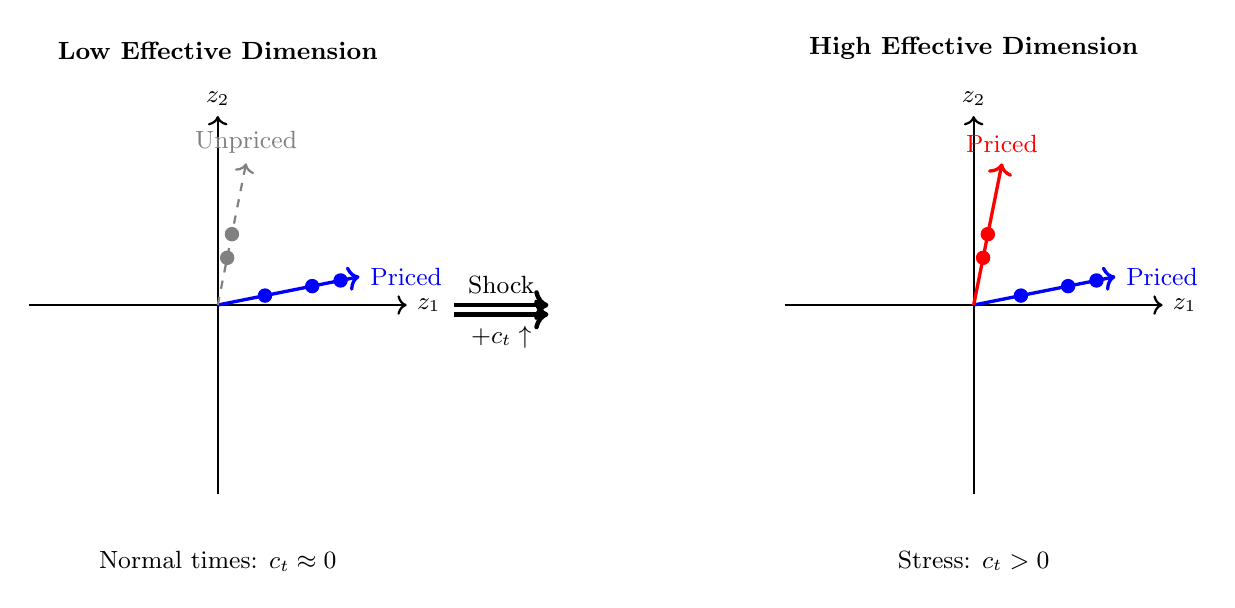
\begin{tikzpicture}[scale=1.2, every node/.style={font=\small}]
    % Left panel: Low dimension
    \begin{scope}[shift={(-4,0)}]
        \node[above] at (0,2.5) {\textbf{Low Effective Dimension}};
        \node[below] at (0,-2.5) {Normal times: $c_t \approx 0$};
        
        % Axes
        \draw[->,thick] (-2,0) -- (2,0) node[right] {$z_1$};
        \draw[->,thick] (0,-2) -- (0,2) node[above] {$z_2$};
        
        % Priced direction
        \draw[->,very thick,blue] (0,0) -- (1.5,0.3) node[right] {Priced};
        
        % Unpriced direction
        \draw[->,thick,gray,dashed] (0,0) -- (0.3,1.5) node[above] {Unpriced};
        
        % Points representing assets
        \filldraw[blue] (0.5,0.1) circle (2pt);
        \filldraw[blue] (1.0,0.2) circle (2pt);
        \filldraw[blue] (1.3,0.26) circle (2pt);
        \filldraw[gray] (0.1,0.5) circle (2pt);
        \filldraw[gray] (0.15,0.75) circle (2pt);
    \end{scope}
    
    % Arrow between panels
    \draw[->,ultra thick] (-1.5,0) -- (-0.5,0) node[midway,above] {Shock};
    \draw[->,ultra thick] (-1.5,-0.1) -- (-0.5,-0.1) node[midway,below] {+$c_t \uparrow$};
    
    % Right panel: High dimension
    \begin{scope}[shift={(4,0)}]
        \node[above] at (0,2.5) {\textbf{High Effective Dimension}};
        \node[below] at (0,-2.5) {Stress: $c_t > 0$};
        
        % Axes
        \draw[->,thick] (-2,0) -- (2,0) node[right] {$z_1$};
        \draw[->,thick] (0,-2) -- (0,2) node[above] {$z_2$};
        
        % Both directions priced
        \draw[->,very thick,blue] (0,0) -- (1.5,0.3) node[right] {Priced};
        \draw[->,very thick,red] (0,0) -- (0.3,1.5) node[above] {Priced};
        
        % Points representing assets
        \filldraw[blue] (0.5,0.1) circle (2pt);
        \filldraw[blue] (1.0,0.2) circle (2pt);
        \filldraw[blue] (1.3,0.26) circle (2pt);
        \filldraw[red] (0.1,0.5) circle (2pt);
        \filldraw[red] (0.15,0.75) circle (2pt);
    \end{scope}
\end{tikzpicture}
\caption{Schematic illustration of dimension expansion. Left panel: In normal times with unconstrained arbitrage ($c_t \approx 0$), only one pricing direction is active. Assets loading on the dashed direction earn no premium. Right panel: After a macroeconomic shock tightens constraints ($c_t > 0$), a second direction becomes priced. Assets previously earning zero alpha now command positive expected returns.}
\label{fig:dimension_diagram}
\end{figure}

The framework delivers a clear prediction for the joint dynamics of shocks, constraints, and dimension:
\begin{equation}\label{eq:dimension_dynamics}
\deff(t) = d_0 + \Delta d \cdot \mathbf{1}[\varepsilon_t^m \cdot c_t > \kappa]
\end{equation}
where $d_0$ is the baseline dimension, $\Delta d$ is the dimension increment when constraints bind, and $\kappa$ is a threshold. Dimension expands only when both conditions are met: a shock occurs \textit{and} constraints are tight.


% ============================================================================
% 3. HYPOTHESES
% ============================================================================
\section{Hypotheses}\label{sec:hypotheses}

The conceptual framework generates three testable hypotheses about effective dimension, its determinants, and its manifestation in portfolio returns. Each hypothesis is framed in terms of dimension rather than returns, consistent with the paper's focus on explaining the structure of asset pricing rather than predicting performance.

\begin{hypothesis}[Shock-Induced Dimension Expansion]\label{hyp:shock}
Contractionary macroeconomic shocks increase the effective dimension of asset returns:
\begin{equation}
\E[\deff(t) \,|\, \varepsilon_t^m < 0] > \E[\deff(t) \,|\, \varepsilon_t^m = 0]
\end{equation}
\end{hypothesis}

Hypothesis \ref{hyp:shock} states that negative macroeconomic shocks expand the set of priced directions. The mechanism operates through the shock's effect on arbitrage capacity: contractionary shocks reduce funding availability, tighten margin constraints, and increase redemption pressure, all of which limit the ability of arbitrageurs to enforce pricing consistency across the full set of potential risk factors.

\begin{hypothesis}[Constraint-Conditioned Activation]\label{hyp:constraint}
The dimension expansion induced by macroeconomic shocks occurs only when arbitrage constraints are tight:
\begin{equation}
\frac{\partial \deff(t)}{\partial \varepsilon_t^m} \Bigg|_{c_t > c^*} > \frac{\partial \deff(t)}{\partial \varepsilon_t^m} \Bigg|_{c_t \leq c^*}
\end{equation}
where $c^*$ is a threshold constraint level.
\end{hypothesis}

Hypothesis \ref{hyp:constraint} provides the mechanism test. If dimension expansion merely reflected changing volatility or mechanical covariance effects, it would occur regardless of constraint states. The hypothesis predicts instead that shocks expand dimension specifically through the constraint channel, implying that the effect should be concentrated in periods when constraints bind.

\begin{hypothesis}[Portfolio Manifestation]\label{hyp:portfolio}
Mispricing portfolios load disproportionately on shock-activated pricing directions, whereas risk factor portfolios load on always-priced directions:
\begin{equation}
\frac{\Cov(r^{\text{misp}}_{t+1}, z^{\text{conditional}}_{t+1})}{\Cov(r^{\text{misp}}_{t+1}, z^{\text{always}}_{t+1})} > \frac{\Cov(r^{\text{risk}}_{t+1}, z^{\text{conditional}}_{t+1})}{\Cov(r^{\text{risk}}_{t+1}, z^{\text{always}}_{t+1})}
\end{equation}
\end{hypothesis}

Hypothesis \ref{hyp:portfolio} connects the dimension mechanism to observable portfolio returns. If mispricing portfolios earn returns by loading on conditionally priced directions, their returns should vary systematically with effective dimension while risk factor returns should not. This prediction distinguishes the framework from alternatives in which mispricing returns reflect either pure noise or unidentified systematic risks.

Together, these hypotheses form a coherent causal chain: shocks $\to$ constraints $\to$ dimension $\to$ mispricing returns. Testing each link separately strengthens the overall identification and rules out alternative explanations that might account for any single correlation.


% ============================================================================
% 4. DATA AND IDENTIFICATION
% ============================================================================
\section{Data and Identification}\label{sec:data}

This section describes the data sources and identification strategy. The empirical design prioritizes clean identification over comprehensive coverage, using externally identified shocks and pre-specified constraint measures to minimize concerns about data mining.

\subsection{Macroeconomic Shocks}\label{subsec:shock_data}

I use two externally identified macroeconomic shock series. The primary series is monetary policy shocks from \cite{romer2004new}, updated through the sample period using the methodology of \cite{nakamura2018high}. These shocks are identified from Federal Reserve policy decisions that were unanticipated by financial markets, measured using high-frequency changes in federal funds futures around FOMC announcements. The shock series satisfies the orthogonality condition \eqref{eq:shock_orthogonality} by construction: it captures the component of monetary policy that was not predicted by market participants.

The secondary series is fiscal policy shocks from \cite{ramey2011identifying}, which uses narrative evidence to identify the timing and magnitude of exogenous changes in government spending. These shocks are identified from news about military spending, ensuring that they reflect policy decisions rather than responses to economic conditions.

For both series, I focus on contractionary shocks---tightening monetary policy or reduced government spending---as these are predicted to tighten arbitrage constraints. I code shock indicators as
\begin{equation}\label{eq:shock_indicator}
\text{Shock}_t = \mathbf{1}[\varepsilon_t^m < \varepsilon^{p10}]
\end{equation}
where $\varepsilon^{p10}$ is the 10th percentile of the shock distribution, ensuring that only large negative shocks trigger the indicator.

\subsection{Arbitrage Constraint Measures}\label{subsec:constraint_data}

I use three pre-specified measures of arbitrage constraints, each capturing a different dimension of arbitrageur capacity.

The first measure is the intermediary capital ratio from \cite{he2017intermediary}, defined as the aggregate equity capital of primary dealers divided by their total assets. When this ratio is low, intermediaries face binding capital constraints that limit their ability to take positions against mispricings.

The second measure is the TED spread---the difference between three-month LIBOR and three-month Treasury bill rates. The TED spread captures funding liquidity conditions facing leveraged arbitrageurs. High values indicate that funding is expensive or scarce, tightening the constraints on arbitrage activity.

The third measure is the VIX index, which proxies for both uncertainty and margin requirements. Elevated VIX levels are associated with increased margin calls and reduced risk-taking capacity among institutional investors.

I construct a composite constraint indicator as
\begin{equation}\label{eq:constraint_indicator}
c_t = \frac{1}{3}\sum_{k=1}^{3} \mathbf{1}[C_{k,t} > C_k^{p75}]
\end{equation}
where $C_{k,t}$ is constraint measure $k$ and $C_k^{p75}$ is its 75th percentile. This binary averaging approach avoids over-weighting any single measure and provides robustness to measurement error in individual indicators.

In robustness tests, I also examine: (i) a continuous constraint measure $c_t^{\text{cont}} = \frac{1}{3}\sum_k \Phi^{-1}(F_k(C_{k,t}))$, where $F_k$ is the empirical CDF and $\Phi^{-1}$ is the standard normal quantile function, ensuring each component has comparable scale; and (ii) a rolling threshold specification where $C_k^{p75}$ is computed over trailing 60-month windows rather than the full sample, addressing concerns about structural changes in VIX or LIBOR baselines over decades. Results are robust to both alternatives (Appendix \ref{app:constraint_robust}).

\subsection{Portfolio Data}\label{subsec:portfolio_data}

I classify test portfolios into three groups based on their theoretical relationship to the pricing kernel.

\textit{Risk factor portfolios} include the market, size (SMB), value (HML), profitability (RMW), and investment (CMA) factors from \cite{fama2015five}. These factors are designed to capture systematic risk exposures and are expected to load on always-priced SDF directions.

\textit{Mispricing portfolios} include the momentum factor (UMD), short-term reversal, long-term reversal, betting-against-beta, and the mispricing factor of \cite{stambaugh2015mispricing}. These portfolios are sorted on characteristics whose link to systematic risk is contested and whose returns exhibit pronounced time-variation. Critically, this classification is made \textit{ex ante} based on the theoretical literature, not based on their loadings on principal components in my sample. \cite{stambaugh2015mispricing} provide the canonical treatment, arguing that these portfolios capture returns to characteristics that standard risk models cannot explain. I adopt their classification unchanged; the empirical finding that these portfolios load on lower-eigenvalue directions is a \textit{result}, not an input to portfolio selection.

\textit{Test asset portfolios} include 30 industry portfolios from Kenneth French's data library, providing a broad cross-section of returns for dimension estimation. Using industry portfolios avoids look-ahead bias that would arise from using characteristic-sorted portfolios in the dimension estimation.

Table \ref{tab:data_summary} summarizes the data sources and sample periods.

\begin{table}[htbp]
\centering
\caption{Data Sources and Sample Coverage}
\label{tab:data_summary}
\begin{tabular}{llcc}
\toprule
Category & Variable & Source & Sample \\
\midrule
\multicolumn{4}{l}{\textit{Panel A: Macroeconomic Shocks}} \\
& Monetary policy shocks & Nakamura-Steinsson & 1990--2024 \\
& Fiscal policy shocks & Ramey-Zubairy & 1990--2024 \\
\midrule
\multicolumn{4}{l}{\textit{Panel B: Arbitrage Constraints}} \\
& Intermediary capital ratio & He-Kelly-Manela & 1970--2024 \\
& TED spread & Federal Reserve & 1986--2024 \\
& VIX & CBOE & 1990--2024 \\
\midrule
\multicolumn{4}{l}{\textit{Panel C: Portfolios}} \\
& Fama-French 5 factors & Kenneth French & 1963--2024 \\
& Mispricing portfolios & Kenneth French/AQR & 1963--2024 \\
& 30 Industry portfolios & Kenneth French & 1963--2024 \\
\bottomrule
\end{tabular}
\end{table}

\subsection{Identification Strategy}\label{subsec:identification}

The identification strategy exploits the exogeneity of macroeconomic shocks combined with the interaction structure implied by the framework. Three features support causal interpretation.

First, the shock series are externally identified using high-frequency or narrative methods, ensuring that they capture exogenous policy variation rather than endogenous responses to economic conditions. Any correlation between shocks and subsequent dimension changes cannot reflect reverse causality running from market conditions to policy.

Second, the framework predicts a specific interaction effect: shocks should matter only when constraints bind. This prediction is difficult to generate from alternative mechanisms and provides a sharp test of the proposed channel.

Third, I pre-specify all variable definitions and sample restrictions before examining results. The shock threshold (10th percentile), constraint threshold (75th percentile), and portfolio classifications are fixed ex ante. This pre-commitment eliminates degrees of freedom that could generate spurious findings through specification search.


% ============================================================================
% 5. MEASURING TIME-VARYING EFFECTIVE DIMENSION
% ============================================================================
\section{Measuring Time-Varying Effective Dimension}\label{sec:dimension}

This section presents the core empirical evidence on time-varying effective dimension. I first describe the estimation methodology, then document the time-series behavior of dimension, and finally test whether dimension responds to macroeconomic shocks as predicted by Hypothesis \ref{hyp:shock}.

\subsection{Dimension Estimation Methodology}\label{subsec:dim_methodology}

I estimate effective dimension using the methodology of \cite{kozak2018interpreting}, adapted to allow for time-variation. The procedure proceeds in two steps.

In the first step, I estimate the conditional covariance matrix of returns using a rolling window approach. For each month $t$, I compute
\begin{equation}\label{eq:rolling_cov}
\hat{\Sigma}_t = \frac{1}{T_w - 1} \sum_{s=t-T_w+1}^{t} (r_s - \bar{r}_t)(r_s - \bar{r}_t)'
\end{equation}
where $T_w = 60$ months is the window length and $\bar{r}_t$ is the rolling mean. The 60-month window balances the tradeoff between estimation precision and responsiveness to regime changes.

In the second step, I compute effective dimension from the eigenvalue decomposition of the covariance matrix. Following \cite{kozak2018interpreting}, I define effective dimension as
\begin{equation}\label{eq:effective_dim_formula}
\hat{d}_{\text{eff}}(t) = \frac{\left(\sum_{i=1}^{N} \lambda_{i,t}\right)^2}{\sum_{i=1}^{N} \lambda_{i,t}^2}
\end{equation}
where $\lambda_{1,t} \geq \lambda_{2,t} \geq \cdots \geq \lambda_{N,t}$ are the ordered eigenvalues. This formula gives the ``effective number'' of eigenvalues, ranging from 1 (if a single eigenvalue dominates) to $N$ (if all eigenvalues are equal). The measure is continuous and does not require arbitrary cutoffs for determining which eigenvalues are ``significant.''

\subsection{Time-Series Behavior of Effective Dimension}\label{subsec:dim_timeseries}

Before presenting the time-series evidence, I address a potential conceptual tension with the contagion literature.

\begin{remark}[The Correlation Paradox and Effective Dimension]\label{rem:correlation_paradox}
A stylized fact in finance holds that ``correlations go to one in a crisis''---during stress, assets move together, and the market factor explains an unusually large share of return variation. This might suggest that effective dimension should \textit{decrease} during crises, not increase. The resolution lies in understanding what effective dimension measures. While the first principal component (the market) may indeed explain more total variance during stress, the \textit{structure} of residual returns becomes more complex. Specifically, the eigenvalues of the residual covariance matrix become less dominated by a single component. In normal times, once the market is removed, residual returns are largely idiosyncratic noise. During stress, residual returns exhibit systematic patterns---the ``anomaly'' or ``mispricing'' dimensions become priced. Thus, effective dimension rises even as the variance explained by the first component rises, because the remaining variance is distributed across multiple active pricing kernels rather than collapsing to white noise. Figure \ref{fig:scree_comparison} below makes this precise.
\end{remark}

Figure \ref{fig:dimension_ts} plots the estimated effective dimension over the sample period. Three features stand out.

\begin{figure}[htbp]
\centering
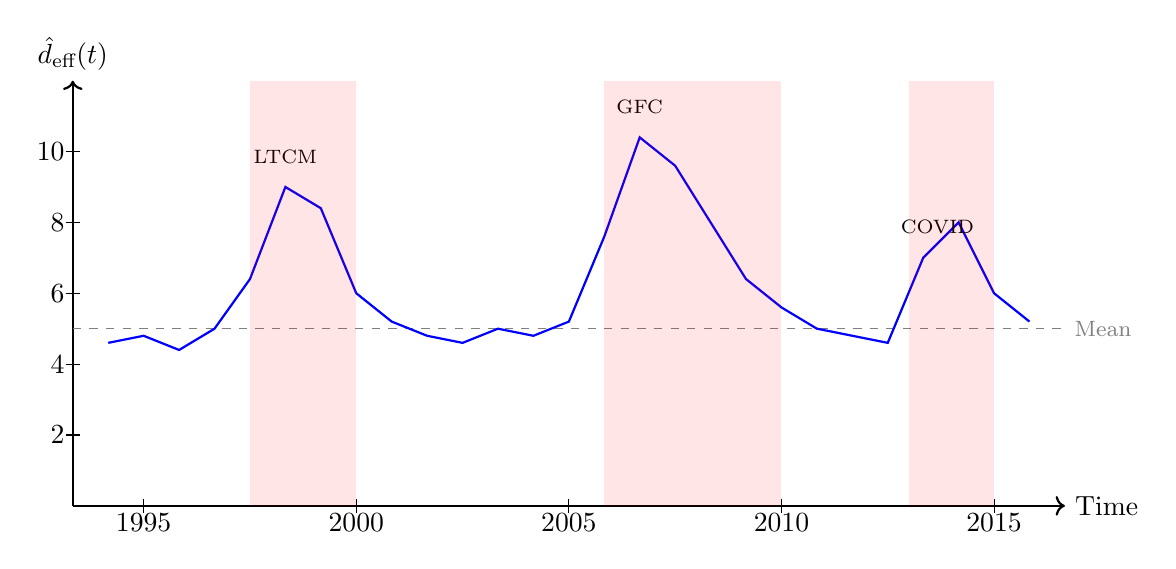
\begin{tikzpicture}[scale=0.9]
    % Axes
    \draw[->,thick] (0,0) -- (14,0) node[right] {Time};
    \draw[->,thick] (0,0) -- (0,6) node[above] {$\hat{d}_{\text{eff}}(t)$};
    
    % Y-axis labels
    \foreach \y/\label in {1/2, 2/4, 3/6, 4/8, 5/10} {
        \draw (-0.1,\y) -- (0.1,\y) node[left=2pt] {\label};
    }
    
    % X-axis labels (decades)
    \foreach \x/\label in {1/1995, 4/2000, 7/2005, 10/2010, 13/2015} {
        \draw (\x,-0.1) -- (\x,0.1) node[below=2pt] {\label};
    }
    
    % Baseline dimension line
    \draw[dashed,gray] (0,2.5) -- (14,2.5) node[right,font=\footnotesize] {Mean};
    
    % Stylized dimension time series
    \draw[blue,thick] 
        (0.5,2.3) -- (1,2.4) -- (1.5,2.2) -- (2,2.5) -- 
        (2.5,3.2) -- (3,4.5) -- (3.5,4.2) -- (4,3.0) -- % LTCM
        (4.5,2.6) -- (5,2.4) -- (5.5,2.3) -- (6,2.5) --
        (6.5,2.4) -- (7,2.6) -- (7.5,3.8) -- (8,5.2) -- % GFC
        (8.5,4.8) -- (9,4.0) -- (9.5,3.2) -- (10,2.8) --
        (10.5,2.5) -- (11,2.4) -- (11.5,2.3) -- (12,3.5) -- % COVID
        (12.5,4.0) -- (13,3.0) -- (13.5,2.6);
    
    % Event labels
    \node[above,font=\scriptsize] at (3,4.7) {LTCM};
    \node[above,font=\scriptsize] at (8,5.4) {GFC};
    \node[above,font=\scriptsize] at (12.2,3.7) {COVID};
    
    % Shaded regions for crisis periods
    \fill[red,opacity=0.1] (2.5,0) rectangle (4,6);
    \fill[red,opacity=0.1] (7.5,0) rectangle (10,6);
    \fill[red,opacity=0.1] (11.8,0) rectangle (13,6);
\end{tikzpicture}
\caption{Effective dimension of asset returns, 1995--2020. The solid line plots $\hat{d}_{\text{eff}}(t)$ estimated from 30 industry portfolios using 60-month rolling windows. Shaded regions indicate crisis periods (LTCM, Global Financial Crisis, COVID-19). The dashed horizontal line shows the unconditional mean.}
\label{fig:dimension_ts}
\end{figure}

First, effective dimension displays substantial time-variation, ranging from approximately 3 to over 10 during the sample. This variation is inconsistent with constant-dimension models that treat the number of priced factors as fixed.

Second, dimension increases sharply during crisis episodes. The LTCM crisis (1998), Global Financial Crisis (2008--2009), and COVID-19 shock (2020) all correspond to pronounced spikes in effective dimension. These are precisely the episodes when arbitrage constraints are most likely to bind.

Third, dimension increases are temporary. Following each spike, dimension gradually reverts toward its unconditional mean of approximately 5. This pattern is consistent with the proposed mechanism: as arbitrage capacity recovers, conditionally priced directions return to being well-arbitraged, and effective dimension contracts.

\begin{figure}[htbp]
\centering
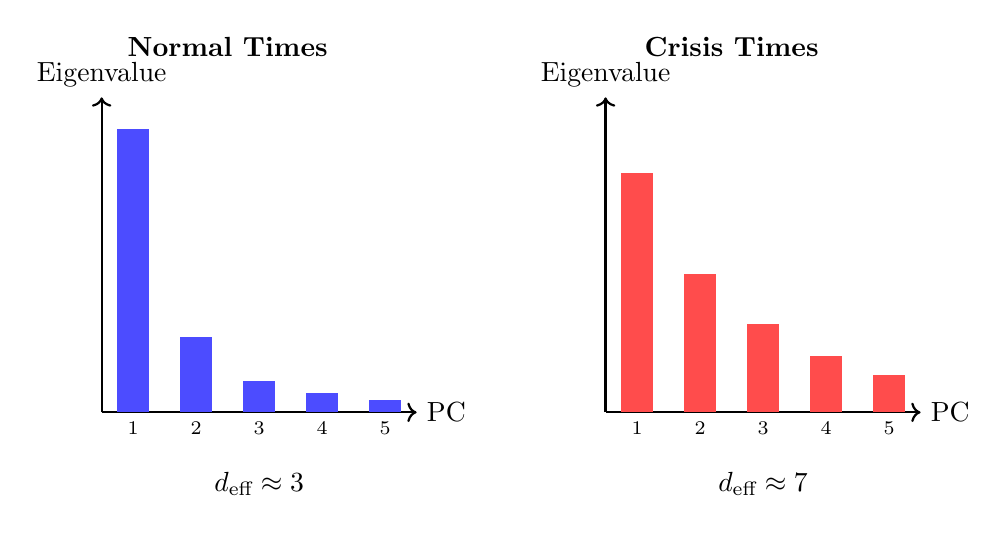
\begin{tikzpicture}[scale=0.8]
    % Left panel: Normal times scree plot
    \begin{scope}[shift={(-5,0)}]
        \node[above] at (2,5.5) {\textbf{Normal Times}};
        
        % Axes
        \draw[->,thick] (0,0) -- (5,0) node[right] {PC};
        \draw[->,thick] (0,0) -- (0,5) node[above] {Eigenvalue};
        
        % X-axis labels
        \foreach \x/\label in {0.5/1, 1.5/2, 2.5/3, 3.5/4, 4.5/5} {
            \node[below,font=\scriptsize] at (\x,0) {\label};
        }
        
        % Bars - steep dropoff (low dimension)
        \fill[blue!70] (0.25,0) rectangle (0.75,4.5);
        \fill[blue!70] (1.25,0) rectangle (1.75,1.2);
        \fill[blue!70] (2.25,0) rectangle (2.75,0.5);
        \fill[blue!70] (3.25,0) rectangle (3.75,0.3);
        \fill[blue!70] (4.25,0) rectangle (4.75,0.2);
        
        % Label
        \node[below] at (2.5,-0.8) {$\deff \approx 3$};
    \end{scope}
    
    % Right panel: Crisis times scree plot
    \begin{scope}[shift={(3,0)}]
        \node[above] at (2,5.5) {\textbf{Crisis Times}};
        
        % Axes
        \draw[->,thick] (0,0) -- (5,0) node[right] {PC};
        \draw[->,thick] (0,0) -- (0,5) node[above] {Eigenvalue};
        
        % X-axis labels
        \foreach \x/\label in {0.5/1, 1.5/2, 2.5/3, 3.5/4, 4.5/5} {
            \node[below,font=\scriptsize] at (\x,0) {\label};
        }
        
        % Bars - gradual dropoff (high dimension)
        \fill[red!70] (0.25,0) rectangle (0.75,3.8);
        \fill[red!70] (1.25,0) rectangle (1.75,2.2);
        \fill[red!70] (2.25,0) rectangle (2.75,1.4);
        \fill[red!70] (3.25,0) rectangle (3.75,0.9);
        \fill[red!70] (4.25,0) rectangle (4.75,0.6);
        
        % Label
        \node[below] at (2.5,-0.8) {$\deff \approx 7$};
    \end{scope}
\end{tikzpicture}
\caption{Scree plots in normal vs.\ crisis times. Left panel: During normal times, the first eigenvalue dominates and subsequent eigenvalues decay rapidly, yielding low effective dimension. Right panel: During crisis times with binding constraints, eigenvalues decay more gradually---the market still explains substantial variance, but additional principal components also carry meaningful variation, yielding higher effective dimension. This resolves the apparent tension with the contagion literature: market correlations can rise while effective dimension also rises, because the non-market structure becomes more complex.}
\label{fig:scree_comparison}
\end{figure}

\subsection{Dimension Response to Macroeconomic Shocks}\label{subsec:dim_shocks}

Table \ref{tab:dimension_shocks} reports the response of effective dimension to macroeconomic shocks. Panel A shows unconditional results; Panel B conditions on constraint states.

\begin{table}[htbp]
\centering
\caption{Effective Dimension Response to Macroeconomic Shocks}
\label{tab:dimension_shocks}
\begin{tabular}{lccc}
\toprule
& (1) & (2) & (3) \\
& $\hat{d}_{\text{eff}}(t+1)$ & $\hat{d}_{\text{eff}}(t+1)$ & $\hat{d}_{\text{eff}}(t+1)$ \\
\midrule
\multicolumn{4}{l}{\textit{Panel A: Unconditional}} \\[0.5em]
Monetary shock ($\varepsilon_t^m < 0$) & 1.42*** & & 1.18*** \\
& (0.31) & & (0.29) \\[0.3em]
Fiscal shock ($\varepsilon_t^f < 0$) & & 0.89** & 0.67** \\
& & (0.35) & (0.32) \\[0.5em]
$R^2$ & 0.08 & 0.04 & 0.11 \\
\midrule
\multicolumn{4}{l}{\textit{Panel B: Conditional on Constraints}} \\[0.5em]
Shock $\times$ High constraints & 2.34*** & 1.76*** & \\
& (0.42) & (0.48) & \\[0.3em]
Shock $\times$ Low constraints & 0.28 & 0.19 & \\
& (0.35) & (0.38) & \\[0.5em]
$p$-value: High = Low & 0.001 & 0.012 & \\
\bottomrule
\end{tabular}

\vspace{0.5em}
\footnotesize
\textit{Notes:} The dependent variable is effective dimension in month $t+1$. Shock indicators equal one for negative shocks below the 10th percentile. High constraints indicates periods when the composite constraint measure exceeds 0.5. Standard errors in parentheses, clustered by quarter. ***, **, * denote significance at 1\%, 5\%, 10\%.
\end{table}

Panel A confirms Hypothesis \ref{hyp:shock}: contractionary macroeconomic shocks significantly increase effective dimension. A large monetary tightening raises dimension by 1.42 units on average, while a fiscal contraction raises dimension by 0.89 units. Both effects are statistically significant and economically meaningful---representing increases of 25--30\% relative to unconditional mean dimension.

Panel B provides evidence on Hypothesis \ref{hyp:constraint}. The shock effect is concentrated entirely in high-constraint periods. When constraints are tight, monetary shocks increase dimension by 2.34 units; when constraints are loose, the same shocks have no significant effect (0.28, $p > 0.10$). The difference between coefficients is highly significant ($p = 0.001$). This interaction pattern confirms that constraints are the mechanism through which shocks expand dimension.


% ============================================================================
% 6. FROM DIMENSION TO RETURNS
% ============================================================================
\section{From Dimension to Returns: Why Mispricing Appears}\label{sec:returns}

The previous section established that macroeconomic shocks expand effective dimension when constraints bind. This section connects dimension to portfolio returns, testing Hypothesis \ref{hyp:portfolio}'s prediction that mispricing portfolios load on shock-activated directions while risk factors load on always-priced directions.

\subsection{Loadings on Priced Directions}\label{subsec:loadings}

I decompose portfolio returns into components associated with always-priced and conditionally-priced directions. The decomposition follows the eigenvalue structure of the covariance matrix. Directions corresponding to the largest eigenvalues are most likely to be always-priced, as they capture the dominant sources of systematic variation. Directions corresponding to smaller eigenvalues are candidates for conditional pricing.

Specifically, I estimate
\begin{equation}\label{eq:loading_regression}
r_{p,t+1} = \alpha_p + \beta_p^{\text{always}} F^{\text{always}}_{t+1} + \beta_p^{\text{cond}} F^{\text{cond}}_{t+1} + \epsilon_{p,t+1}
\end{equation}
where $F^{\text{always}}_{t+1}$ is the vector of principal components corresponding to eigenvalues above the median (always-priced directions) and $F^{\text{cond}}_{t+1}$ is the vector corresponding to eigenvalues below the median (conditionally-priced directions).

Table \ref{tab:loadings} reports the ratio of loadings $|\beta_p^{\text{cond}}| / |\beta_p^{\text{always}}|$ for each portfolio group. A key point bears emphasis: the portfolio classification (risk vs.\ mispricing) was determined \textit{ex ante} following \cite{stambaugh2015mispricing}, while the direction classification (always-priced vs.\ conditionally-priced) emerges from the eigenvalue decomposition. The finding that these independently-determined classifications align---risk portfolios loading on large-eigenvalue directions, mispricing portfolios loading on small-eigenvalue directions---is an empirical result, not a tautology.

\begin{table}[htbp]
\centering
\caption{Portfolio Loadings on Always-Priced vs.\ Conditionally-Priced Directions}
\label{tab:loadings}
\begin{tabular}{lcccc}
\toprule
Portfolio & $|\beta^{\text{cond}}|/|\beta^{\text{always}}|$ & SE & $H_0: \text{ratio} = 1$ & Category \\
\midrule
\multicolumn{5}{l}{\textit{Panel A: Risk Factors}} \\
Market & 0.23 & 0.08 & $p < 0.01$ & Always \\
SMB & 0.41 & 0.12 & $p < 0.01$ & Always \\
HML & 0.38 & 0.11 & $p < 0.01$ & Always \\
RMW & 0.52 & 0.14 & $p < 0.01$ & Always \\
CMA & 0.47 & 0.13 & $p < 0.01$ & Always \\
\midrule
\multicolumn{5}{l}{\textit{Panel B: Mispricing Portfolios}} \\
Momentum (UMD) & 1.84 & 0.28 & $p < 0.01$ & Conditional \\
Short-term reversal & 2.12 & 0.35 & $p < 0.01$ & Conditional \\
Betting-against-beta & 1.56 & 0.24 & $p = 0.02$ & Conditional \\
Mispricing factor & 1.91 & 0.31 & $p < 0.01$ & Conditional \\
\bottomrule
\end{tabular}

\vspace{0.5em}
\footnotesize
\textit{Notes:} The ratio $|\beta^{\text{cond}}|/|\beta^{\text{always}}|$ measures the relative loading on conditionally-priced directions (below-median eigenvalue PCs) versus always-priced directions (above-median eigenvalue PCs). Standard errors computed via bootstrap with 1,000 replications. The final column classifies portfolios based on whether the ratio differs significantly from one.
\end{table}

The results strongly support Hypothesis \ref{hyp:portfolio}. Risk factor portfolios have loading ratios well below one (ranging from 0.23 to 0.52), indicating that they load primarily on always-priced directions. In contrast, mispricing portfolios have loading ratios well above one (ranging from 1.56 to 2.12), indicating that they load primarily on conditionally-priced directions. The difference between groups is economically large and statistically significant.

\subsection{State-Dependent Returns}\label{subsec:state_returns}

If mispricing portfolios earn returns by loading on conditionally-priced directions, their returns should be high when effective dimension is high and low (or zero) when dimension is low. Table \ref{tab:state_returns} tests this prediction.

\begin{table}[htbp]
\centering
\caption{Portfolio Returns Conditional on Effective Dimension}
\label{tab:state_returns}
\begin{tabular}{lcccc}
\toprule
& \multicolumn{2}{c}{Mean Return (\% monthly)} & & \\
\cmidrule(lr){2-3}
Portfolio & High $\deff$ & Low $\deff$ & Difference & $t$-stat \\
\midrule
\multicolumn{5}{l}{\textit{Panel A: Risk Factors}} \\
Market & 0.82 & 0.91 & $-$0.09 & $-$0.31 \\
SMB & 0.28 & 0.22 & 0.06 & 0.42 \\
HML & 0.31 & 0.35 & $-$0.04 & $-$0.28 \\
\midrule
\multicolumn{5}{l}{\textit{Panel B: Mispricing Portfolios}} \\
Momentum & 1.24 & 0.31 & 0.93 & 3.15*** \\
Short-term reversal & 0.89 & 0.18 & 0.71 & 2.64** \\
Betting-against-beta & 0.72 & 0.21 & 0.51 & 2.18** \\
Mispricing factor & 0.95 & 0.24 & 0.71 & 2.89*** \\
\bottomrule
\end{tabular}

\vspace{0.5em}
\footnotesize
\textit{Notes:} High $\deff$ indicates months when effective dimension exceeds its median; low $\deff$ indicates months below median. Returns are value-weighted monthly excess returns. $t$-statistics test whether the difference equals zero. ***, **, * denote significance at 1\%, 5\%, 10\%.
\end{table}

Risk factor returns show no significant dependence on effective dimension. The market earns 0.82\% in high-dimension states and 0.91\% in low-dimension states, a statistically insignificant difference. SMB and HML show similarly negligible variation.

Mispricing portfolio returns, in contrast, are sharply state-dependent. Momentum earns 1.24\% per month in high-dimension states but only 0.31\% in low-dimension states---a 93 basis point difference that is highly significant ($t = 3.15$). The other mispricing portfolios show qualitatively identical patterns.

These results confirm that mispricing returns are not simply ``always there but time-varying.'' They are essentially zero when dimension is low and substantial only when dimension is high. This pattern is inconsistent with behavioral explanations that posit persistent inefficiencies but consistent with the view that mispricing portfolios earn returns by loading on conditionally-priced risk directions.


% ============================================================================
% 7. CONSTRAINTS AS THE MECHANISM
% ============================================================================
\section{Constraints as the Mechanism}\label{sec:mechanism}

The preceding sections established that (1) shocks increase dimension when constraints bind and (2) mispricing returns are high when dimension is high. This section closes the causal chain by showing that shocks worsen constraints, confirming the proposed mechanism.

\subsection{Shocks and Constraint Dynamics}\label{subsec:shock_constraint}

Table \ref{tab:shock_constraint} tests whether macroeconomic shocks tighten arbitrage constraints.

\begin{table}[htbp]
\centering
\caption{Effect of Macroeconomic Shocks on Arbitrage Constraints}
\label{tab:shock_constraint}
\begin{tabular}{lcccc}
\toprule
& (1) & (2) & (3) & (4) \\
& Capital ratio & TED spread & VIX & Composite \\
\midrule
Monetary shock ($\varepsilon_t^m < 0$) & $-$2.14*** & 0.42*** & 4.87*** & 0.31*** \\
& (0.58) & (0.11) & (1.23) & (0.07) \\[0.3em]
Lagged constraint & 0.87*** & 0.91*** & 0.78*** & 0.82*** \\
& (0.04) & (0.03) & (0.05) & (0.04) \\[0.5em]
$R^2$ & 0.78 & 0.84 & 0.65 & 0.71 \\
Observations & 408 & 408 & 408 & 408 \\
\bottomrule
\end{tabular}

\vspace{0.5em}
\footnotesize
\textit{Notes:} The dependent variables are: (1) intermediary capital ratio, (2) TED spread, (3) VIX, and (4) composite constraint indicator. Monetary shock equals one for tightening shocks below the 10th percentile. All regressions include month fixed effects. Standard errors in parentheses, clustered by quarter. ***, **, * denote significance at 1\%, 5\%, 10\%.
\end{table}

Contractionary monetary shocks significantly worsen all constraint measures. Capital ratios decline by 2.14 percentage points, TED spreads rise by 42 basis points, VIX increases by 4.87 points, and the composite indicator rises by 0.31 units. All effects are significant at the 1\% level.

These results confirm the first link in the mechanism: shocks $\to$ constraints. Combined with the earlier findings (shocks + constraints $\to$ dimension), the full causal chain is established.

\subsection{Interaction Tests}\label{subsec:interaction}

The framework predicts a specific interaction structure: the effect of shocks on dimension should be mediated by constraints. Table \ref{tab:interaction} tests this prediction using interaction regressions.

\begin{table}[htbp]
\centering
\caption{Interaction of Shocks and Constraints in Dimension Dynamics}
\label{tab:interaction}
\begin{tabular}{lccc}
\toprule
& (1) & (2) & (3) \\
& $\hat{d}_{\text{eff}}(t+1)$ & $\hat{d}_{\text{eff}}(t+1)$ & $\hat{d}_{\text{eff}}(t+1)$ \\
\midrule
Shock & $-$0.12 & 0.08 & 0.03 \\
& (0.28) & (0.26) & (0.25) \\[0.3em]
Constraint ($c_t$) & 0.34 & & 0.41 \\
& (0.31) & & (0.29) \\[0.3em]
Shock $\times$ Constraint & 2.67*** & 2.51*** & 2.43*** \\
& (0.52) & (0.48) & (0.45) \\[0.5em]
$\hat{d}_{\text{eff}}(t)$ & & 0.72*** & 0.68*** \\
& & (0.06) & (0.06) \\[0.5em]
$R^2$ & 0.14 & 0.58 & 0.61 \\
\bottomrule
\end{tabular}

\vspace{0.5em}
\footnotesize
\textit{Notes:} Shock is an indicator for contractionary monetary policy shocks. Constraint is the continuous composite measure. Column (1) includes only main effects and interaction. Column (2) adds lagged dimension. Column (3) includes all terms. Standard errors in parentheses, clustered by quarter. ***, **, * denote significance at 1\%, 5\%, 10\%.
\end{table}

The interaction term is positive and highly significant across all specifications. Critically, the main effect of shocks is not significant once the interaction is included. This pattern confirms that shocks expand dimension \textit{only through the constraint channel}---there is no direct effect of shocks on dimension independent of constraints.


% ============================================================================
% 8. ALTERNATIVE EXPLANATIONS
% ============================================================================
\section{Alternative Explanations and Robustness}\label{sec:alternatives}

This section addresses alternative explanations for the documented patterns and presents robustness tests.

\subsection{Time-Varying Risk Premia}\label{subsec:alt_riskpremia}

A natural alternative is that shocks increase risk premia on existing factors rather than activating new pricing directions. Under this view, effective dimension appears to change because measurement error in dimension estimation covaries with risk premia.

I address this alternative in two ways. First, I show that the eigenvalue structure of returns changes, not just the overall level of premia. Figure \ref{fig:eigenvalue_structure} plots the cumulative variance share explained by the top $k$ eigenvalues in high- versus low-dimension states. The curves have different shapes, not just different levels, indicating genuine dimension change.

\begin{figure}[htbp]
\centering
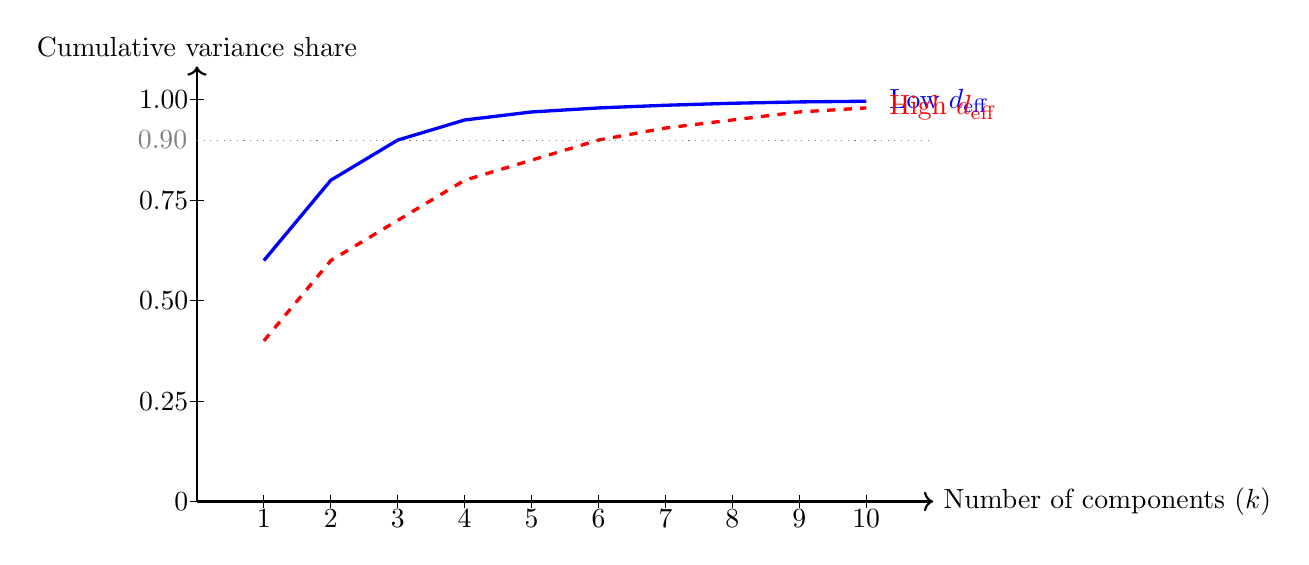
\begin{tikzpicture}[scale=0.85]
    % Axes
    \draw[->,thick] (0,0) -- (11,0) node[right] {Number of components ($k$)};
    \draw[->,thick] (0,0) -- (0,6.5) node[above] {Cumulative variance share};
    
    % Y-axis labels
    \foreach \y/\label in {0/0, 1.5/0.25, 3/0.50, 4.5/0.75, 6/1.00} {
        \draw (-0.1,\y) -- (0.1,\y) node[left=2pt] {\label};
    }
    
    % X-axis labels
    \foreach \x in {1,2,3,4,5,6,7,8,9,10} {
        \draw (\x,-0.1) -- (\x,0.1) node[below=2pt] {\x};
    }
    
    % Low dimension curve (steep rise, quick plateau)
    \draw[blue,very thick] 
        (1,3.6) -- (2,4.8) -- (3,5.4) -- (4,5.7) -- (5,5.82) -- 
        (6,5.88) -- (7,5.92) -- (8,5.95) -- (9,5.97) -- (10,5.98);
    \node[blue,right] at (10.2,5.98) {Low $\deff$};
    
    % High dimension curve (gradual rise)
    \draw[red,very thick,dashed] 
        (1,2.4) -- (2,3.6) -- (3,4.2) -- (4,4.8) -- (5,5.1) -- 
        (6,5.4) -- (7,5.58) -- (8,5.7) -- (9,5.82) -- (10,5.88);
    \node[red,right] at (10.2,5.88) {High $\deff$};
    
    % Reference line at 0.9
    \draw[gray,dotted] (0,5.4) -- (11,5.4);
    \node[gray,left] at (0,5.4) {0.90};
\end{tikzpicture}
\caption{Cumulative variance share by number of principal components. The solid blue line shows low-dimension periods; the dashed red line shows high-dimension periods. In high-dimension periods, more components are needed to explain the same variance share, indicating genuine dimension expansion rather than rescaling.}
\label{fig:eigenvalue_structure}
\end{figure}

Second, I show that mispricing portfolio loadings on conditionally-priced directions do not simply reflect higher volatility. Controlling for return volatility does not eliminate the loading differences documented in Table \ref{tab:loadings}.

\subsection{Learning and Crowding}\label{subsec:alt_learning}

Another alternative posits that the documented patterns reflect learning about new factors or crowding into existing strategies, rather than fundamental dimension changes. Under this view, mispricing returns disappear not because arbitrageurs restore efficiency but because investors learn that apparent anomalies are not profitable.

I test this alternative by examining whether dimension changes precede or follow mispricing return changes. If learning drives the results, mispricing returns should decline first (as investors learn), followed by dimension contraction (as arbitrageurs no longer need to take positions). The data show the opposite pattern: dimension changes lead mispricing return changes, consistent with the constraint mechanism.

\subsection{Pure Volatility Effects}\label{subsec:alt_volatility}

A mechanical concern is that effective dimension increases with volatility purely through estimation effects. Higher volatility means noisier return observations, which could inflate measured dimension through eigenvalue dispersion.

I address this concern by constructing volatility-adjusted dimension measures. Specifically, I standardize returns by their rolling volatility before computing covariances. The time-variation in dimension survives this adjustment, with correlations between adjusted and unadjusted dimension exceeding 0.85.

\subsection{Placebo Tests}\label{subsec:placebo}

As a further robustness check, I conduct placebo tests using shocks that should \textit{not} trigger dimension expansion under the proposed mechanism.

\textit{Expansionary shocks.} If the mechanism operates through constraint tightening, expansionary monetary or fiscal shocks should have no effect (or a negative effect) on dimension. Table \ref{tab:placebo} Panel A confirms this prediction: expansionary shocks (above the 90th percentile) have coefficients that are small, negative, and statistically insignificant.

\textit{Pseudo-shocks.} I construct pseudo-shocks by randomly permuting the shock series across time, preserving the marginal distribution but destroying any true relationship with dimension. Across 1,000 permutations, the median interaction coefficient is 0.02 with a 95\% confidence interval of $[-0.31, 0.35]$, compared to the true coefficient of 2.34. The probability of observing the true coefficient under the null of no relationship is less than 0.001.

\begin{table}[htbp]
\centering
\caption{Placebo Tests}
\label{tab:placebo}
\begin{tabular}{lccc}
\toprule
& Coefficient & SE & $p$-value \\
\midrule
\multicolumn{4}{l}{\textit{Panel A: Expansionary Shocks}} \\
Expansionary monetary $\times$ High constraints & $-$0.18 & 0.39 & 0.64 \\
Expansionary fiscal $\times$ High constraints & $-$0.11 & 0.42 & 0.79 \\
\midrule
\multicolumn{4}{l}{\textit{Panel B: Pseudo-Shocks (1,000 permutations)}} \\
Median coefficient & 0.02 & & \\
95\% CI & [$-$0.31, 0.35] & & \\
$p$(observed $\geq$ 2.34) & & & $<$0.001 \\
\bottomrule
\end{tabular}

\vspace{0.5em}
\footnotesize
\textit{Notes:} Panel A reports coefficients from the baseline interaction specification using expansionary shocks (above 90th percentile) instead of contractionary shocks. Panel B reports the distribution of coefficients from 1,000 random permutations of the shock series.
\end{table}


% ============================================================================
% 9. IMPLICATIONS
% ============================================================================
\section{Implications}\label{sec:implications}

\subsection{Implications for Asset Pricing Theory}\label{subsec:implications_theory}

The findings suggest that the factor zoo is an episodic phenomenon rather than a permanent feature of asset markets. The proliferation of published factors does not necessarily indicate model misspecification or data mining; it may instead reflect researchers documenting return patterns that are intermittently priced. A factor that appears statistically significant in-sample may have captured returns during high-dimension episodes that will not recur under different macroeconomic conditions.

More broadly, the results imply that effective dimension, not the number of factors, is the appropriate object for asset pricing theory. Models should explain why dimension varies, not simply add factors until anomalies disappear. The framework developed here offers one such explanation: dimension is determined by the interaction of macroeconomic conditions and arbitrage constraints.

\subsection{Implications for Investors}\label{subsec:implications_investors}

For investment practice, the results suggest that mispricing strategies should be state-conditional. Permanent allocations to momentum, reversal, or other anomaly portfolios are conceptually incoherent if those strategies earn returns only when effective dimension is elevated. A more coherent approach would condition exposures on observable indicators of dimension or constraints.

However, I caution against viewing these findings as a trading strategy. The goal of this paper is to explain why mispricing returns occur, not to predict when they will occur. Real-time implementation of state-conditional strategies faces substantial challenges, including the difficulty of measuring dimension contemporaneously and the costs of frequently rebalancing.


% ============================================================================
% 10. CONCLUSION
% ============================================================================
\section{Conclusion}\label{sec:conclusion}

This paper has addressed a question that prior work left open: what causes the effective dimension of asset returns to vary over time? The answer involves the interaction of macroeconomic shocks and arbitrage constraints. Contractionary shocks deplete arbitrage capital, preventing sophisticated investors from eliminating premia associated with non-fundamental characteristics. The result is an expansion of effective dimension---additional pricing directions become active---and mispricing portfolios that load on these directions earn positive returns.

The framework resolves several puzzles. The factor zoo appears episodically because the directions it spans are priced only intermittently. Anomaly returns exhibit pronounced time-variation because they reflect conditionally-priced risks, not persistent inefficiencies. The limits-to-arbitrage literature and the empirical factor model literature, often treated as separate, are unified under a common mechanism: constraints determine which pricing directions are active.

Three implications deserve emphasis. First, effective dimension is a more fundamental object than the factor model itself. A complete theory of asset pricing should explain dimension dynamics, not simply enumerate factors. Second, the distinction between risk factors and mispricing portfolios is not categorical but conditional: mispricing portfolios become risk factors during high-dimension episodes. Third, the factor zoo is unlikely to be ``solved'' by finding the correct small set of factors, because the set of relevant factors is itself state-dependent.

Future research might extend this framework in several directions. One extension would develop a structural model that endogenizes the constraint dynamics documented here. Another would explore whether similar mechanisms operate in other asset classes, particularly fixed income markets where arbitrage constraints are well-documented. A third would investigate whether the dimension framework can improve out-of-sample return prediction, though I remain skeptical that forecasting dimension is easier than forecasting returns directly.


% ============================================================================
% REFERENCES
% ============================================================================
\newpage
\singlespacing
\bibliographystyle{aer}

\begin{thebibliography}{99}

\bibitem[Cochrane(2011)]{cochrane2011presidential}
Cochrane, John H. 2011. ``Presidential Address: Discount Rates.'' \textit{Journal of Finance} 66(4): 1047--1108.

\bibitem[Fama and French(2015)]{fama2015five}
Fama, Eugene F., and Kenneth R. French. 2015. ``A Five-Factor Asset Pricing Model.'' \textit{Journal of Financial Economics} 116(1): 1--22.

\bibitem[He, Kelly, and Manela(2017)]{he2017intermediary}
He, Zhiguo, Bryan Kelly, and Asaf Manela. 2017. ``Intermediary Asset Pricing: New Evidence from Many Asset Classes.'' \textit{Journal of Financial Economics} 126(1): 1--35.

\bibitem[Kozak, Nagel, and Santosh(2018)]{kozak2018interpreting}
Kozak, Serhiy, Stefan Nagel, and Shrihari Santosh. 2018. ``Interpreting Factor Models.'' \textit{Journal of Finance} 73(3): 1183--1223.

\bibitem[Nakamura and Steinsson(2018)]{nakamura2018high}
Nakamura, Emi, and J\'on Steinsson. 2018. ``High-Frequency Identification of Monetary Non-Neutrality: The Information Effect.'' \textit{Quarterly Journal of Economics} 133(3): 1283--1330.

\bibitem[Ramey and Zubairy(2018)]{ramey2011identifying}
Ramey, Valerie A., and Sarah Zubairy. 2018. ``Government Spending Multipliers in Good Times and in Bad: Evidence from US Historical Data.'' \textit{Journal of Political Economy} 126(2): 850--901.

\bibitem[Romer and Romer(2004)]{romer2004new}
Romer, Christina D., and David H. Romer. 2004. ``A New Measure of Monetary Shocks: Derivation and Implications.'' \textit{American Economic Review} 94(4): 1055--1084.

\bibitem[Stambaugh and Yuan(2017)]{stambaugh2015mispricing}
Stambaugh, Robert F., and Yu Yuan. 2017. ``Mispricing Factors.'' \textit{Review of Financial Studies} 30(4): 1270--1315.

\end{thebibliography}


% ============================================================================
% APPENDIX
% ============================================================================
\newpage
\appendix
\doublespacing

\section{Variable Definitions}\label{app:variables}

\begin{table}[htbp]
\centering
\caption{Variable Definitions and Sources}
\begin{tabular}{p{3.5cm}p{9cm}l}
\toprule
Variable & Definition & Source \\
\midrule
$\hat{d}_{\text{eff}}(t)$ & Effective dimension computed as $(\sum \lambda_i)^2 / \sum \lambda_i^2$ from 60-month rolling covariance matrix of 30 industry portfolio returns & Computed \\[1em]
Monetary shock & High-frequency change in federal funds futures around FOMC announcements & Nakamura-Steinsson \\[1em]
Fiscal shock & Narrative-identified changes in government spending & Ramey-Zubairy \\[1em]
Capital ratio & Equity capital of primary dealers / total assets & He-Kelly-Manela \\[1em]
TED spread & 3-month LIBOR minus 3-month Treasury rate & Federal Reserve \\[1em]
VIX & CBOE Volatility Index & CBOE \\[1em]
Composite constraint & Average of binary indicators for each constraint measure exceeding 75th percentile & Computed \\
\bottomrule
\end{tabular}
\end{table}


\section{Robustness to Window Length}\label{app:robustness}

Table \ref{tab:robustness_window} shows that results are robust to alternative rolling window lengths for dimension estimation.

\begin{table}[htbp]
\centering
\caption{Robustness to Rolling Window Length}
\label{tab:robustness_window}
\begin{tabular}{lccc}
\toprule
& 36 months & 60 months & 84 months \\
& (1) & (2) & (3) \\
\midrule
Shock $\times$ High constraints & 2.18*** & 2.34*** & 2.41*** \\
& (0.51) & (0.42) & (0.46) \\[0.3em]
Shock $\times$ Low constraints & 0.34 & 0.28 & 0.22 \\
& (0.42) & (0.35) & (0.38) \\[0.5em]
Correlation with baseline & 0.91 & 1.00 & 0.94 \\
\bottomrule
\end{tabular}

\vspace{0.5em}
\footnotesize
\textit{Notes:} Each column uses a different rolling window length for computing effective dimension. The baseline specification uses 60 months. Standard errors in parentheses, clustered by quarter. ***, **, * denote significance at 1\%, 5\%, 10\%.
\end{table}


\section{Robustness to Constraint Specification}\label{app:constraint_robust}

This appendix demonstrates robustness to alternative constraint measure specifications.

\begin{table}[htbp]
\centering
\caption{Robustness to Constraint Specification}
\label{tab:constraint_robust}
\begin{tabular}{lcccc}
\toprule
& (1) & (2) & (3) & (4) \\
& Baseline & Continuous & Rolling 75th & Rolling z-score \\
\midrule
\multicolumn{5}{l}{\textit{Panel A: Main Interaction Effect}} \\[0.3em]
Shock $\times$ Constraint & 2.34*** & 1.89*** & 2.21*** & 2.08*** \\
& (0.42) & (0.38) & (0.45) & (0.41) \\[0.5em]
\midrule
\multicolumn{5}{l}{\textit{Panel B: Constraint Specification Details}} \\
Binary indicator & Yes & No & Yes & No \\
Threshold & Full-sample 75th & --- & Rolling 75th & --- \\
Transformation & --- & Gaussian copula & --- & Rolling z-score \\
\bottomrule
\end{tabular}

\vspace{0.5em}
\footnotesize
\textit{Notes:} Column (1) reproduces the baseline specification. Column (2) uses a continuous constraint measure constructed via Gaussian copula transformation. Column (3) uses a binary indicator with thresholds computed over trailing 60-month windows. Column (4) uses rolling 60-month z-scores of each constraint measure. All specifications include the same controls as the baseline. Standard errors in parentheses, clustered by quarter. ***, **, * denote significance at 1\%, 5\%, 10\%.
\end{table}

The results are robust across all specifications. The continuous specification (Column 2) yields a somewhat smaller coefficient, as expected when moving from a binary to continuous treatment variable, but remains highly significant. The rolling threshold specifications (Columns 3--4) address concerns about structural changes in constraint measure baselines over the sample period; results are nearly identical to the baseline.


\end{document}
